\section{Transition systems}
\label{sec:ordinary-transition-systems}
    Transition systems are well established semantic models for both sequential and concurrent systems. A transition system can be viewed as a directed graph, called a state transition graph, whose vertices are states and edges are transitions between states. We may consider a transition system, as shown in Figure \ref{fig:transition-system}, where we have four states $s_{1}$, $s_{2}$, $s_{3}$, and $s_{4}$, for example, representing a program changing a value of a variable at different times of its execution. We also have four transitions, two of which are labeled $a$ and another two which are labeled $b$. We can also have the same label $a$ for both events, giving rise to the notion of \emph{autoconcurrency}. These four transitions, represent two instructions of a program that change the state of the machine from the source of its arrow to its corresponding target. This is formalized by using a transition relation. We will refer to this transition system as the \emph{interleaving square}, similar to what has been done by Pratt \cite{Pratt00Sculptures} and van Glabbeek \cite{Glabbeek06HDA}. We will use the same notation and definitions as Winskel and Nielsen in \cite{winskel95modelsCategory}.
    
    \begin{figure}[ht]
        \centering
        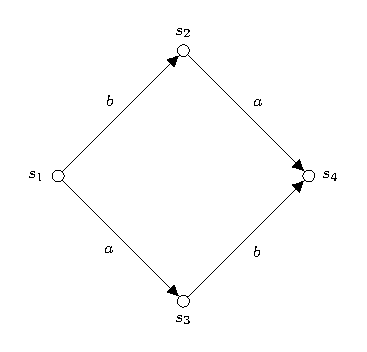
\includegraphics[scale=1.1]{Figures/2.Models-for-concurrency/transition-system.pdf}
        \captionof{figure}[A transition system.]{A transition system with four states, $s_{1}, s_{2}, s_{3}$, and $s_{4}$, and four transitions, two of which are labeled $a$ and the other two are labeled $b$. These four transitions present the interleaving of two instructions. The interleaving is namely the permutation of all possible executions of these two instructions. This transition system is called the interleaving square because of the way the interleaving of two instructions form a square.}
        \label{fig:transition-system}
      
    \end{figure}
    
    \begin{definition}[Transition system \cite{winskel95modelsCategory}]\label{def:transition-system}
        A transition system is a structure ($\mathcal{S}, i, \mathcal{L}, Tran$) where,
        \begin{itemize}
            \item $\mathcal{S}$ is a set of states with initial state i,
            \item $\mathcal{L}$ is a set of labels, and
            \item $Tran \subseteq \mathcal{S} \times \mathcal{L} \times \mathcal{S}$ is the transition relation
        \end{itemize}
    \end{definition}
    
    We will write $s \xrightarrow{a} s'$ to indicate  that $(s,a,s') \in Tran$.
    
    Morphisms between transition systems often describe the relationships between processes. These kind of relations are described by Winskel and Nielsen in \cite{winskel95modelsCategory}, where one process may be a component of another or perhaps one process may refine another process. By defining morphisms as simulations between transition systems, we are able to describe the relationship between processes. For example, a simulation is where a transition system $\mathcal{T}$ simulates a transition system $\mathcal{T}^{'}$, meaning that when $\mathcal{T}^{'}$ can execute some action $a$ then there must exists an $a$ in $\mathcal{T}$ that can be executed.
    
    \begin{definition}[Morphism of transition systems \cite{winskel95modelsCategory}]\label{def:morphism-of-transition-system}
        A morphism from one transition system, $\mathcal{T}$, to another, $\mathcal{T}^{'}$ , will be a pair $(\sigma, \lambda)$ in which
        \begin{itemize}
            \item $\sigma$ is a function from the states of $\mathcal{T}$ to those of $\mathcal{T}^{'}$ .
            \item $\lambda$ is a partial function from the labels of $\mathcal{T}$ to those of $\mathcal{T}^{'}$ such that for any transition $s \xrightarrow{a} s'$ of $\mathcal{T}$ if $\lambda(a)$ is defined, then $\sigma(s) \xrightarrow{\lambda(a)} \sigma(s')$ is a transition of $\mathcal{T}^{'}$ ; otherwise, if $\lambda(a)$ is undefined, then $\sigma(s) = \sigma(s')$.
        \end{itemize}
    \end{definition}
    
    In our notation, we have used $\mathcal{L}$ to stand for the set of labels for events, as well as to stand for the actual set of those events. However, sometimes it might be useful to make a distinction between the events themselves and to explicitly give a labeling as a function. For instance, this is important when treating \emph{relabeling} which leads to categorical fibrational situations \cite{winskel95modelsCategory}. To make the distinction between labels of events and the actual events clearer, we will replace $\mathcal{L}$ with $E$ and refer to its elements as \emph{events}.
    
    \begin{definition}[Labeled transition system \cite{winskel95modelsCategory}]\label{def:labeled-transition-system}
        A \emph{labeled} transition system consists of a transition system $\mathcal{T}$ = ($\mathcal{S}, i, E, Tran$) together with a set $\mathcal{L}$ of labels, and a function $l: E \rightarrow \mathcal{L}$. We denote it by ($\mathcal{T}$, $\mathcal{L}$, $l$).
    \end{definition}
    
    \begin{definition}[Morphism of labeled transition systems \cite{winskel95modelsCategory}]\label{def:morphisms-labeled-transition-system}
        A morphism, ($\sigma,\tau, \lambda$) : ($\mathcal{T}$, $\mathcal{L}$, $l$) $\rightarrow$ ($\mathcal{T}^{'}$, $\mathcal{L}^{'}$, $l^{'}$) between labeled transition systems consists of a morphism ($\sigma, \tau$) : $\mathcal{T} \rightarrow \mathcal{T}^{'}$ between the underlying transition systems together with a partial function $\lambda : \mathcal{L} \rightarrow \mathcal{L}^{'}$ such that $l' \circ \tau = \lambda \circ l$.
    \end{definition}

    %We will extend on the notion of transition systems to consider "\emph{idle}" transitions as shown in Figure \ref{fig:idle-transition-system}. It is convenient to introduce "\emph{idle}" transitions, associated with any state. Idle transitions help simplify the definition of morphisms between transition systems. By adopting the notation in \cite{winskel95modelsCategory}, it allows us to view the partial function from a set $\mathcal{L}$ to a set $\mathcal{L}^{'}$ as a total function $\lambda : \mathcal{L} \rightarrow \mathcal{L}^{'} \cup \{*\}$, where we will follow the notation that $*$ is a distinguished element standing for "\emph{undefined}". As done by Winskel in \cite{winskel95modelsCategory}, we will reflect the representation of $*$ in our notation $\lambda : \mathcal{L} \rightarrow_{*} \mathcal{L}^{'}$, for a partial function $\lambda$ from $\mathcal{L}$  to $\mathcal{L}^{'}$. 
    
    %\begin{figure}[ht]
    %    \centering
    %    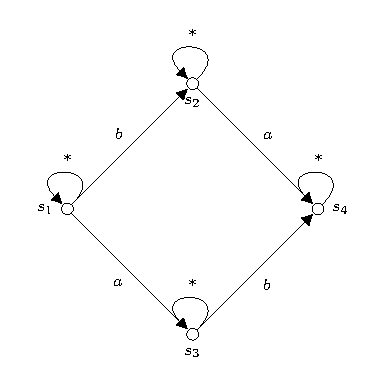
\includegraphics[scale=1.3]{Figures/2.Models-for-concurrency/idle-transition-system.pdf}
    %    \captionof{figure}[An idle transition system.]{A transition system with four states, $s_{1}, s_{2}, s_{3}$, and $s_{4}$, and eight transitions, two of which are labeled $a$, another two which are labeled $b$ and the remaining are loops labeled $*$. The paths with $a$ and $b$ represent the interleaving of two instructions. The interleaving is namely the permutation of all possible executions of these two instructions. While, transitions labelled $*$ refer to the possible inaction of a transition system.}
    %    \label{fig:idle-transition-system}
    %\end{figure}
    
    %This representation will also be reflected in our notation $\lambda : \mathcal{L} \rightarrow_{*} \mathcal{L}^{'}$, for a partial function $\lambda$ from $\mathcal{L}$  to $\mathcal{L}^{'}$. 
    %We define idle transition systems as in \cite{winskel95modelsCategory}.
    
    %\begin{definition}[Idle transition systems \cite{winskel95modelsCategory}]\label{def:idle-transition-system}
    %    Let $\mathcal{T}$ = ($\mathcal{S}, i, \mathcal{L}, Tran$) be a transition system. An idle transition of $\mathcal{T}$ consists of ($s, *, s$) and $s \in \mathcal{S}$ such that
    %    \begin{center}
    %        $Tran_{*} = Tran \cup \{(s,*,s)\ |\ s \in \mathcal{S}\}$.
    %    \end{center}
    %\end{definition}
    
    %We may also define morphisms between idle transition systems as follows:
    
    %\begin{definition}[Morphisms of idle transition systems \cite{winskel95modelsCategory}]\label{def:morphisms-of-idle-transition-system}
    %    Let $\mathcal{T}$ = ($\mathcal{S}, i, \mathcal{L}, Tran$) and $\mathcal{T}^{'}$ = ($\mathcal{S}^{'}, i^{'}, \mathcal{L}^{'}, Tran^{'}$) be transition systems. A morphism $f : \mathcal{T} \rightarrow \mathcal{T}^{'}$ is a pair $f = (\sigma, \lambda)$ where
    %    \begin{itemize}
    %        \item $\sigma : \mathcal{S} \rightarrow \mathcal{S}^{'}$
    %        \item $\lambda : \mathcal{L} \rightarrow \mathcal{L}^{'}$ are such that $\sigma(i)$ = $i'$ and $(s,a,s') \in Tran \Rightarrow (\sigma(s),\lambda(a),\sigma(s')) \in Tran^{'}_{*}$.
    %    \end{itemize}
    %\end{definition}
    
    %If a transition with label $a$ in $\mathcal{T}$ is undefined, then we want a transition with label $\lambda(a)$ in $\mathcal{T}^{'}$ to also be undefined. We will consider this as a transition representing inaction. With the introduction of idle transitions, morphisms on transition systems can be described as preserving transitions and the initial state. Lastly, we will also stress, as done in \cite{winskel95modelsCategory}, that an idle transition ($s, *, s$) represents inaction, and is to be distinguished from the action expressed by a transition ($s, a, s$) for a label \emph{a}. From now on, when referring to transition systems we mean idle transition systems with the extension of morphisms of transition systems considering idle transitions.
    
    We write $\allTS$ for the category of transition systems. Also, we name $\allTS_{E}$ its subcategory where we restrict to transition systems labeled on an alphabet $E$. The alphabet $E$ can be considered the same as the set of events $E$. The notion of transition systems and of morphisms between them is clearly related to directed graphs, labeled directed graphs, and labeled transition systems, but we will need to consider labeled cubical sets, which we will not do here. However, we will introduce precubical sets\footnote{In topology, the difference between cubical and precubical sets are similar to that of simplicial and presimplicial sets. The differences are subtle and will not be considered here. The distinction between cubical and precubical sets is presented in \cite{Goubault95PhDThesis}.} in Section \ref{sec:higher-dimensional-automata}.